\begin{figure}
    \centering
    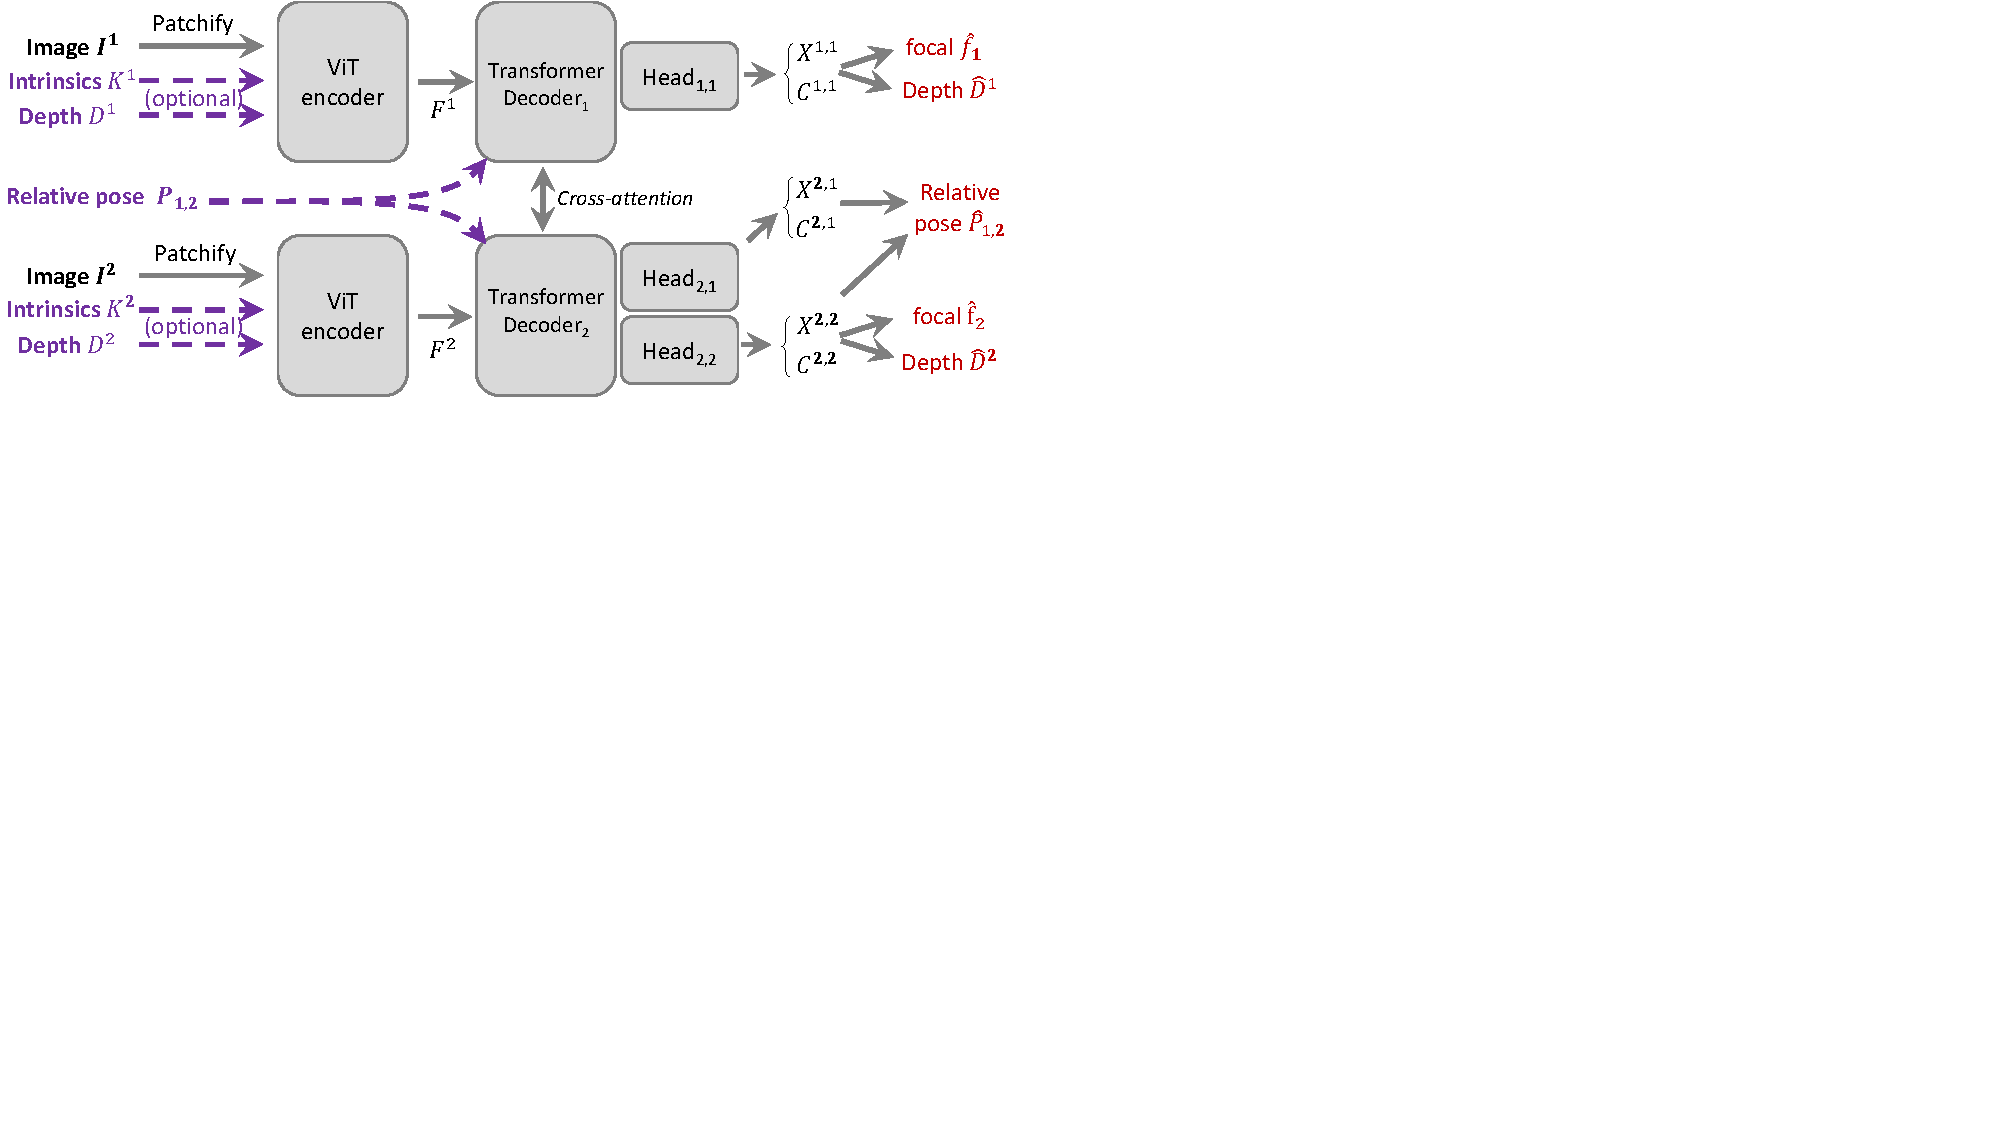
\includegraphics[width=\linewidth,trim=0 350 480 0,clip]{figures/pow3r_overview.pdf} \\[-0.3cm]
    \caption{\textbf{Overview of the model architecture.} 
    Following \duster{}~\cite{wang2024dust3r}, images are encoded then decoded with a ViT backbone into pointmaps, from which focals, depthmaps and relative pose can be extracted.
    \ours{} introduces optional inputs to guide the regression with prior knowledge about the camera intrinsics and depth (fed into the encoder) and the pose (into the decoder).
    } 
    \label{fig:overview}
    \vspace{-0.2cm}
\end{figure}


\section{Methodology}
\label{sec:method}

We aim to train a network $\mathcal{F}$ that can take two input images $I^1,I^2\in \mathbb{R}^{W\times H\times 3}$ of a given static scene and any subset of auxiliary information $\Omega \subseteq \{K_1,K_2,P_{1,2},\D{1},\D{2}\}$, in order to regress a 3D reconstruction of the scene.
Here, $K_1,K_2\in\mathbb{R}^{3\times 3}$ are camera intrinsics, 
$P_{1,2}\in\mathbb{R}^{4\times 4}$ denote the relative pose between the two cameras, 
and $\D{1},\D{2} \in\mathbb{R}^{W\times H}$ are depthmaps with associated masks $M^1,M^2\in\{0,1\}^{W\times H}$ specifying pixels with valid depth data
(\ie masks are possibly sparse).
The network $\mathcal{F}$ is tasked to regress several pointmaps from which the camera intrinsic and extrinsic parameters as well as the dense depthmaps can be straightforwardly extracted for both images as described below. %

\myparagraph{Pointmaps.} 
For each pixel $(i,j)$ in an image $I$, we assume there exists a corresponding single 3D point $X_{i,j}$, where $X\in\R^{W\times H \times 3}$ is a \emph{pointmap}. 
Given camera intrinsics $K$ and a depthmap $D$, we can compute $X_{i,j}=K^{-1} [iD_{i,j}, jD_{i,j}, D_{i,j}]$ in the camera coordinate system.
In the following, we denote as $\X{n}{m}$ the pointmap of image $\I{n}$ expressed in the coordinate system of camera $\I{m}$. 
To swap the coordinate system from camera $\I{k}$ to camera $\I{m}$, we have $X^{n,k} = P_{m,k} X^{n,m}$ where $P_{m,k}=P_k P_m^{-1}$.




\subsection{Overall architecture}

We follow the recently proposed \duster{} framework~\cite{wang2024dust3r}.
\duster{} is a breakthrough foundation model based on vision transformers (ViT) that can regress two 3D pointmaps $\X{1}{1}, \X{2}{1}$ given solely two unposed and uncalibrated input images.
Nevertheless, \duster{}'s inability to leverage potentially available information about cameras or depth %
limits its practical use.
To remedy these drawbacks, we enhance the original \duster{} network $\mathcal{F}$ in two ways.

First, we introduce specific modules to incorporate any subset of extra information such as  camera intrinsics, camera poses and depthmaps seamlessly into \duster{}.
Second, we predict an additional pointmap $\X{2}{2}$, which represents the pointmap of image $\I2$ in its own coordinate system.
Predicting three pointmaps offers further capabilities, namely the possibility of recovering all information about \emph{both} cameras in a single forward pass, as explained in \cref{sec:applications}.
We first describe the overall architecture, see \cref{fig:overview}, and then detail the dedicated modules to inject auxiliary information.


\myparagraph{Encoder.} 
We use a shared ViT encoder to encode both images independently. 
In addition to $I$, the encoder can receive auxiliary information about intrinsics $K$ and depth $D$ for each image.
For the two input images $I^1$, $I^2$ and their respective auxiliary information $\Omega_1 \in \sigma(\{K_1,D_1\}), \Omega_2 \in \sigma(\{K_2,D_2\})$, where $\sigma$ denotes the set of all subsets, the encoder processes the information in a Siamese manner:
\begin{equation}
  F^1 = \text{Encoder}(I^1,\Omega_1), ~~ F^2 = \text{Encoder}(I^2,\Omega_2).
\end{equation}

\myparagraph{Decoder.}
Likewise, the network has two decoders, each with its corresponding head, one predicting $X^{1,1}$ and the other one estimating $X^{2,1}$ and $X^{2,2}$. 
Both decoders communicate via cross-attention between their own tokens and the outputs of the previous block of the other decoder. 
Each decoder may receive the relative pose $P_{12}$ as additional input or not. 
Assume we provide the auxiliary information $\Omega_D \in \sigma(\{P_{12}\})$ at the $i$-th block of both decoders:
\begin{eqnarray}
  G_i^1 = \text{DecoderBlock}^1_{i}\left(G_{i-1}^1, G_{i-1}^2, \Omega_D\right), \nonumber \\
  G_i^2 = \text{DecoderBlock}^2_{i}\left(G_{i-1}^2, G_{i-1}^1, \Omega_D\right),
\end{eqnarray}
After $B$ decoder blocks in each branch,
the head regresses several pointmaps and their associated confidence map:
\begin{eqnarray}
  X^{1,1}, C^{1,1} = \text{Head}^1\left(G_B^1\right), \nonumber \\
  X^{2,1}, X^{2,2}, C^{2,1}, C^{2,2} = \text{Head}^2\left(G_B^2\right).
\end{eqnarray}
Unlike \duster{} which uses a DPT head~\cite{dpt}, here we employ a linear head for both $\text{Head}^1$ and $\text{Head}^2$ %
as it is more efficient and performs similarly.


\myparagraph{3D Regression Loss.} 
Following \duster{}, we supervise the model to minimize the distance between ground-truth and predicted pointmaps in a scale-invariant manner, allowing the model to train on multiple datasets with various scales.
The regression loss between predicted and ground-truth pointmaps (resp. $\X{n}{m}$ and $\Xgt{n}{m}$) at pixel $(i,j)$ is defined as $\lreg_{i,j}(n,m)=\Vert \X{n}{m}_{i,j}/\z_m  - \Xgt{n}{m}_{i,j}/\zgt_m \Vert$, where $\z_m,\zgt_m$ serve as scale normalizer.
That is, $\z_m$ is the average norm of all valid 3D points expressed in coordinate system of image $\I{m}$, \ie  $\z_1=\Z(\X{1}{1} \cup \X{2}{1})$,  $\z_2=\Z(\X{2}{2})$ and likewise for $\zgt_1,\zgt_2$, with $\Z(X)=\text{mean}(\{\Vert X_{i,j} \Vert\, | i,j \in \valid_X\})$ and $\valid_X$ the set of valid pixels. 

\myparagraph{Confidence-aware loss.} 
The model jointly learns to predict a confidence level $\C{n,m}_{i,j}$ of each pixel $(i,j)$.
The confidence-aware regression loss for a given pointmap $\X{n}{m}$ can be expressed as the 3D regression loss $\lreg$ weighted by the confidence map:
\begin{equation}
  \lconf(n,m) = \sum_{i,j\in\valid} \C{n,m}_{i,j} \lreg_{i,j}(n,m) - \alpha \log \C{n,m}_{i,j},
\label{eq:conf_loss}
\end{equation}
with $\alpha=0.2$. This loss penalizes the model less when the prediction is not accurate on harder areas, encouraging the model to extrapolate.
The final loss is expressed as
\begin{equation}
  \mathcal{L} = \lconf(1,1) + \lconf(2,1) + \beta \lconf(2,2),
\end{equation}
where $\beta$ is a hyper-parameter typically set to $\beta=1$. 

\begin{figure}
    \centering
    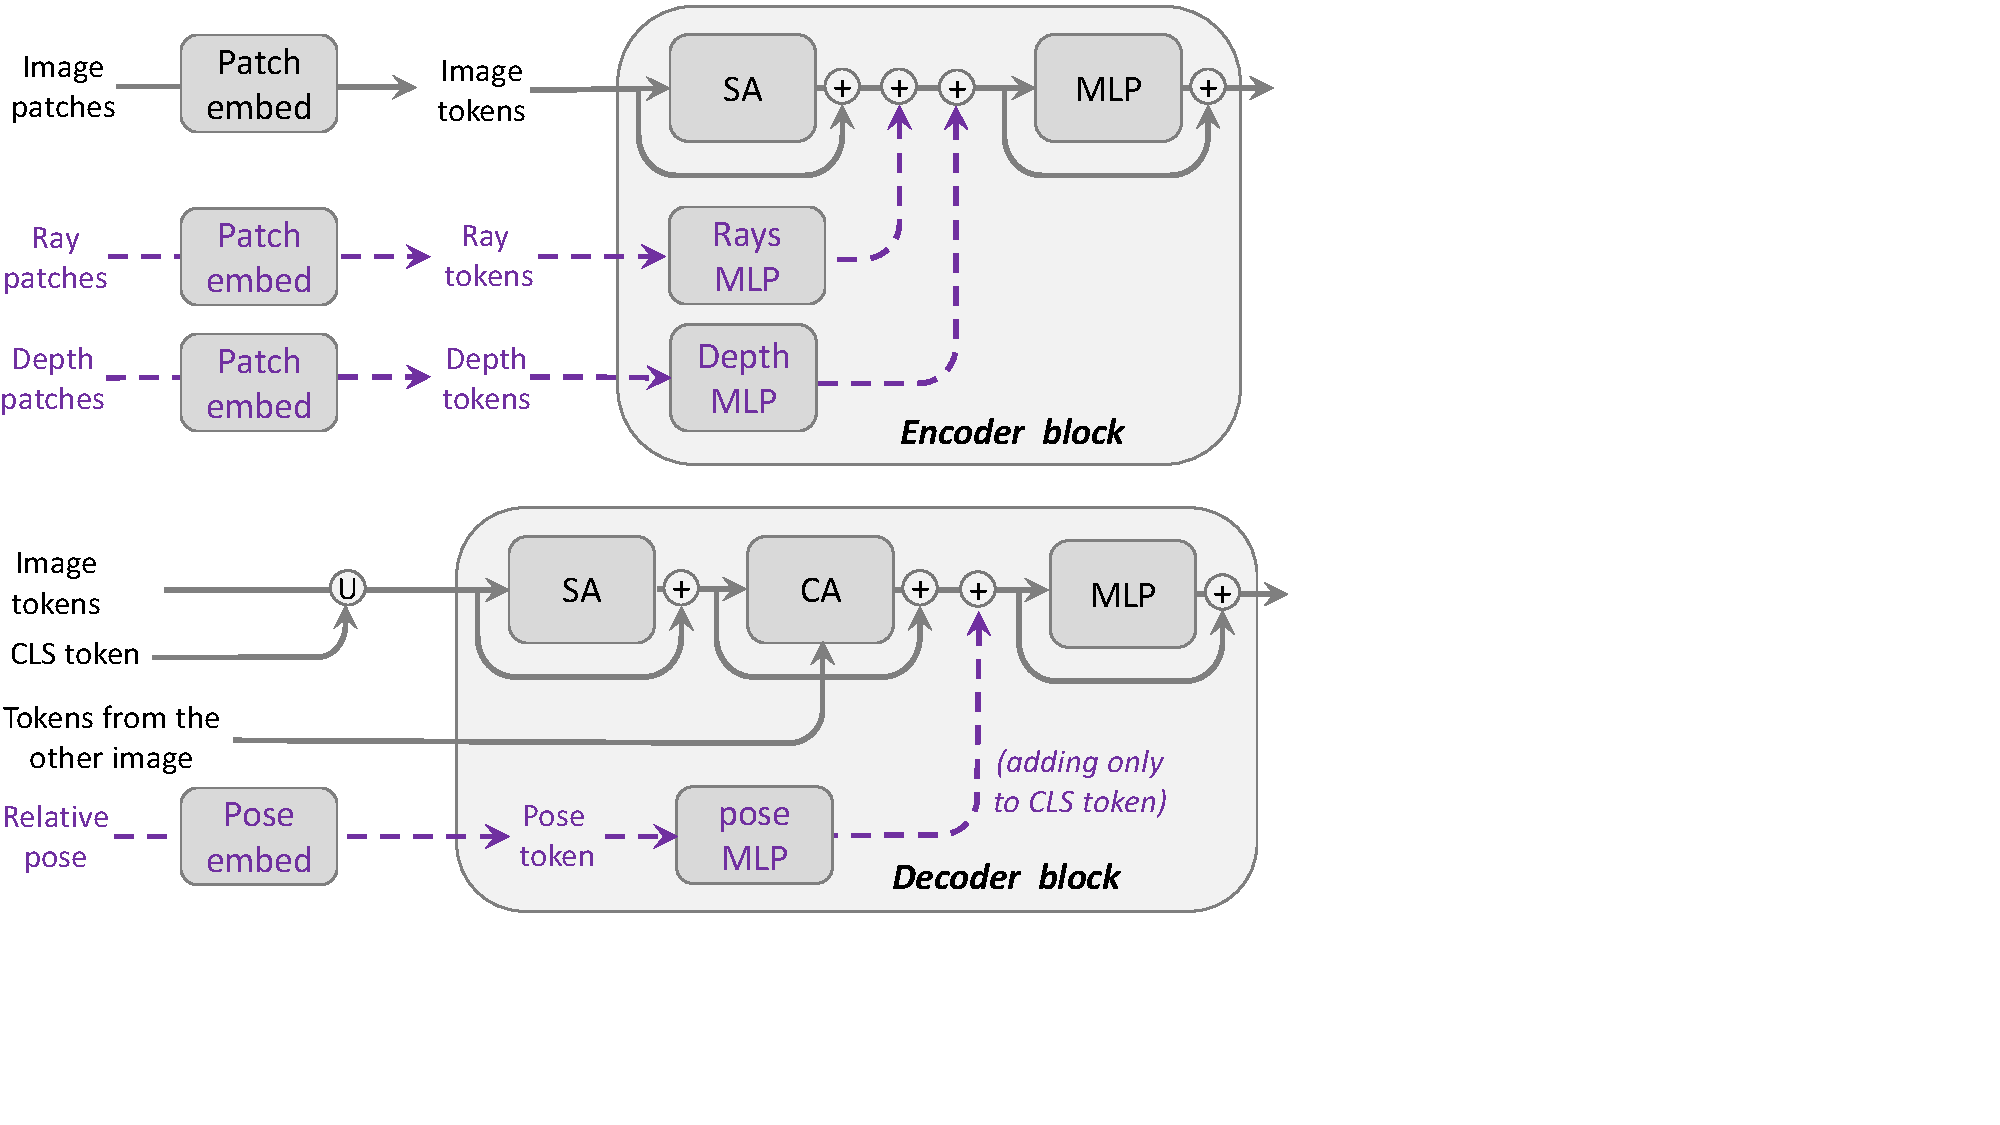
\includegraphics[width=0.9\linewidth,trim=0 100 330 0,clip]{figures/pow3r_blocks.pdf} \\[-0.3cm]
    \caption{\textbf{Architecture for injecting auxiliary modalities.} \textit{Top:} injection of optional intrinsics and depth into the encoder. Intrinsics are encoded into ray patches, sparse depth is %
    patchified. Each of these modalities goes into a block-specific MLP and are token-wise added in the middle of the transformer block.
    \textit{Bottom:} injection of optional relative pose into the decoder. The relative pose is fed to a first embedding layer followed by an MLP. This token is added to the CLS token of the decoder after the self-attention (SA) and cross-attention (CA), but before the MLP.
    Experiments show that injection in the first block only suffices.}
    \vspace{-0.4cm}
    \label{fig:inject}
\end{figure}


\begin{figure*}
    \centering
    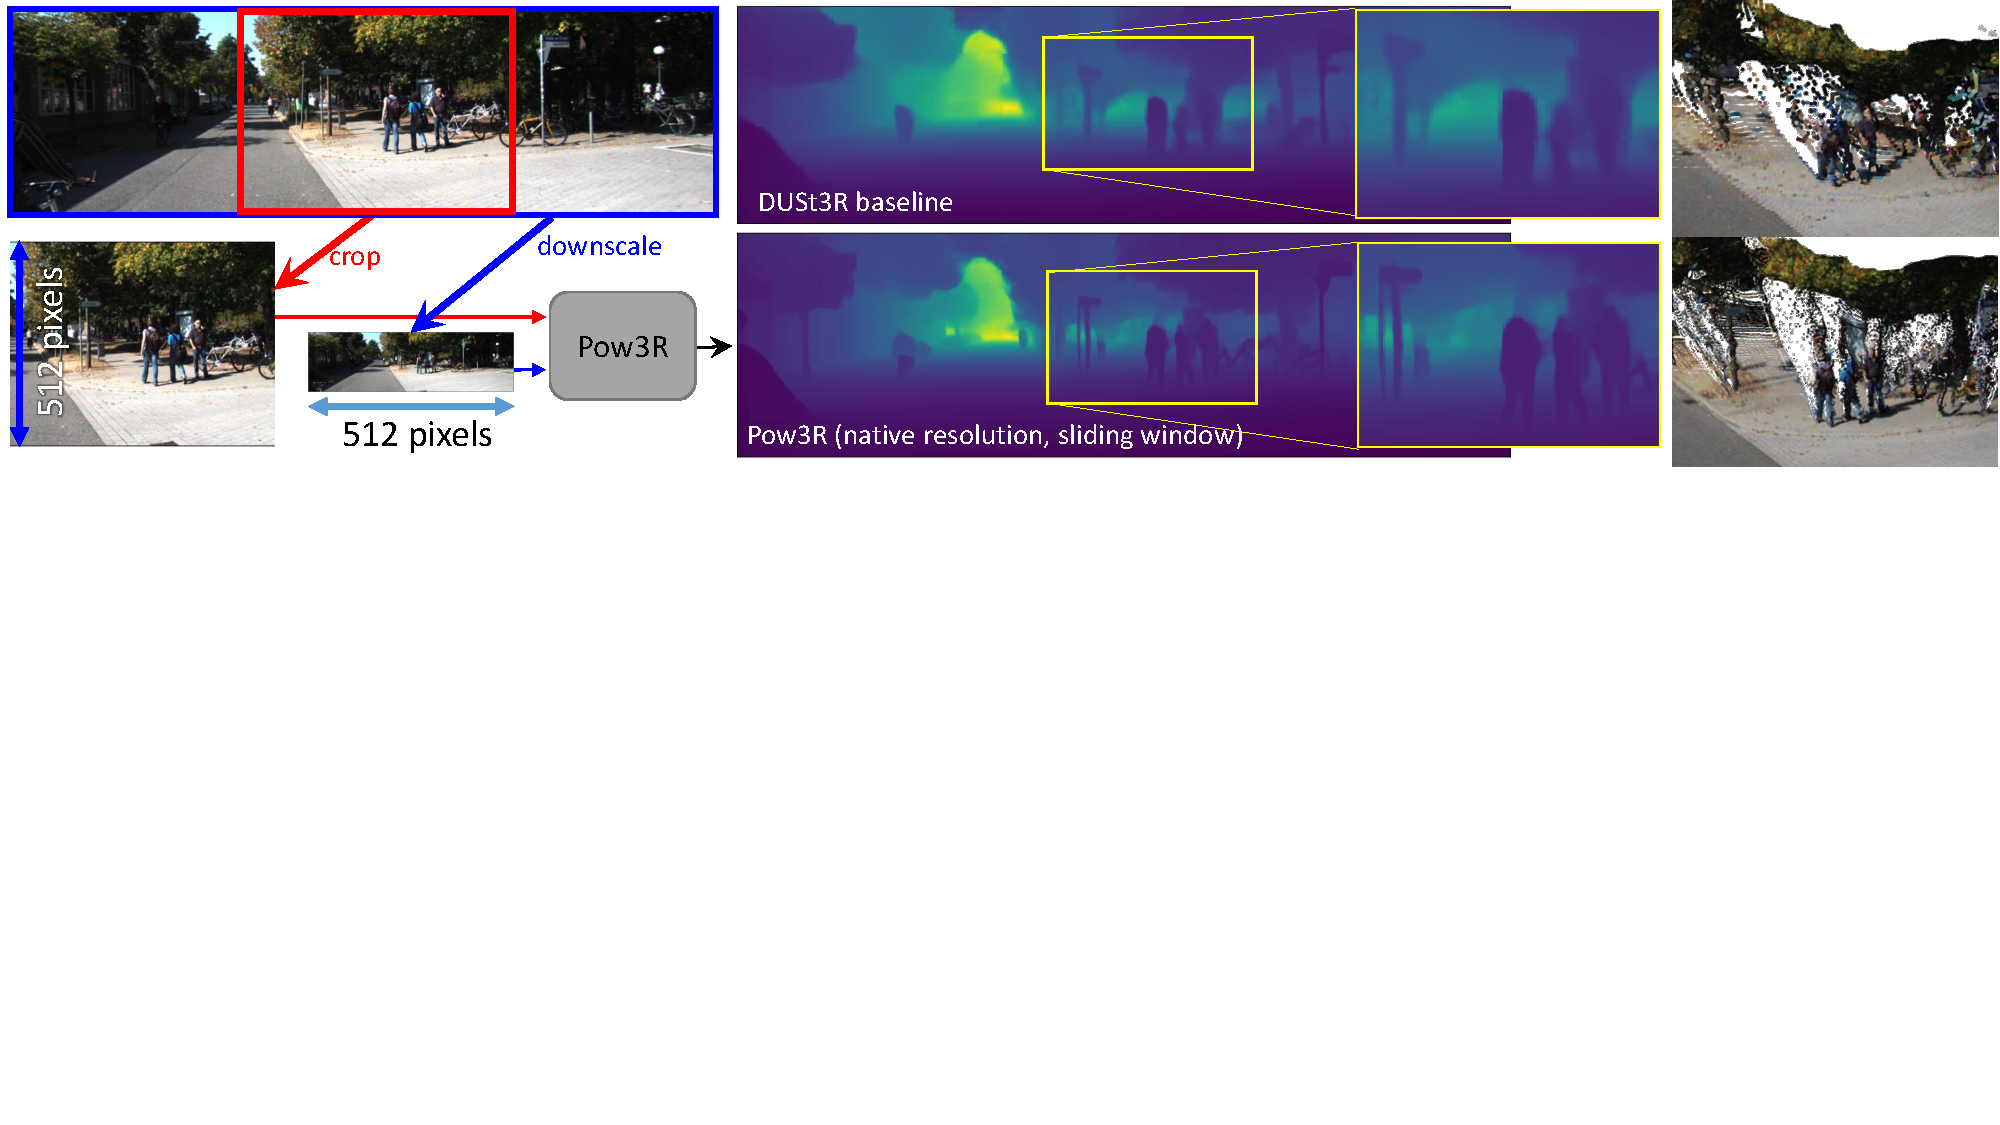
\includegraphics[width=1\linewidth, trim=0 320 0 0, clip]{figures/highres.pdf} \\[-0.3cm]
    \caption{\textbf{Native resolution example.} Methods like DUSt3R require centered principal point and would thus downscale the image to its training resolution, leading to blurry prediction (top). With camera intrinsics input, we can process any crop in the image leading to native resolution prediction (bottom row), for example by dividing the image into 4 crops, that are independently process as the first input image, while the second input image of the network is set to the downscaled image.  
    }
    \vspace{-0.2cm}
    \label{fig:native_ex}  
\end{figure*}

\subsection{Adding Versatile Conditioning}

The knowledge of auxiliary information can significantly enhance 3D predictions at test time.
Our model leverages up to five different modalities, which include two intrinsics $K_1,K_2$, two depthmaps $D^1,D^2$ for each image and the relative pose $P_{12}$.
To condition the output on it, we first embed the auxiliary information using dedicated MLPs and then inject these embeddings at different points in the pipeline.

We discuss different options in this regard. 
In the first strategy, denoted as `\embed{}', we simply add the auxiliary embeddings to the token embeddings before the first transformer block, as would be done for standard positional embeddings~\cite{vit}.
In the second strategy, denoted as `\inject{n}', we instead insert dedicated MLPs for each modality in a subset of $n$ transformer blocks, as shown in \cref{fig:inject}.
Our experiments show that `\inject{1}' performs slightly better than `\embed{}' and similarly with `\inject{n}', where $n>1$, see \cref{sec:ablations}.
We now describe how to compute the initial embeddings for each specific modality.


\myparagraph{Intrinsics.} 
Following~\cite{raydiffusion}, we generate camera rays from the intrinsic matrix $K\in\R^{3\times 3}$, thereby establishing a direct correspondence between RGB pixels and rays. 
The ray at pixel location $(i,j)$ is computed as $K^{-1} [i, j, 1]$ and encodes the viewing direction of that pixel \wrt the current camera pose.
This allows us to potentially process non-centered crops and hence to perform inference in higher image resolutions, see \cref{sec:applications}.
Similarly to RGB inputs, we patchify and embed dense rays and provide them to the encoder.



\myparagraph{Depthmaps / Point Clouds.} 
Given a depthmap $\D{}$ and its sparsity mask $M$, we first normalize $D'=D/\Z(D)$ to handle any depth ranges at train and test time. 
As for RGB and rays, we patchify the stacked maps $[D',M]\in\R^{W\times H\times 2}$ and compute patch embeddings, which are then fed to the encoder.
By jointly patchifying the depth and its valid mask we can handle any level of sparsity. %

\myparagraph{Camera Pose.} 
Given the relative pose $P_{12}=[R_{12}|t_{12}]$, we normalize the translation scale as $t'_{12} = t_{12} / \Vert t_{12} \Vert$ since our output is unscaled. %
Unlike depthmaps or camera intrinsics, the camera pose cannot be expressed as a dense pixel map. %
Rather, camera pose affects the whole pixels between two images, so the embedding is instead added to the global CLS token of both decoders. %










\subsection{Downstream Tasks}
\label{sec:applications}

\myparagraph{Depthmaps.} 
In the pointmap representation, the $z$-axis of $\X{1}{1},\X{2}{2}$ directly corresponds to the depthmaps of the first and second image, respectively.
Note that \duster{} only outputs $\X{1}{1}$, hence it requires two forward passes of the pairs $(\I1, \I2)$ and $(\I2, \I1)$ to extract both depthmaps.

\myparagraph{High-resolution processing.}
A limitation of \duster{} is that it is trained for a specific resolution and does not generalize to larger resolutions.
A simple fix would be to include higher resolutions during training, but (i) many datasets do not provide high-resolution ground-truths, and (ii) the training cost could become prohibitive.
\ours{}, in contrast, can handle crops natively given camera intrinsics of the crop, as these provide the crop position information (\ie via focal length and principal point).
We can thus perform prediction in a sliding window fashion, yielding predictions matching any target resolution by simple stitching.
Comparison between standard and higher resolution processing are shown in \cref{fig:native_ex}.
Note that prediction for each crop may have a different scale, by design, and cannot be stitched directly.
We find that simply computing the median scale factor in overlapping areas is sufficient, and we blend the overlapping regions based on confidence without further post-processing.

\myparagraph{Focal Estimation.} 
Similar to \duster{}, we can recover focals for both input images from pointmap $\X{1}{1}$ and $\X{2}{2}$ with the robust Weiszfeld fast iterative solver~\cite{Plastria2011Weiszfeld}.
Similar to depthmap prediction, \duster{} needs to infer $(I_2,I_1)$ in order to compute the focal of the second image, while \ours{} predicts them in a single pass.

\myparagraph{Relative Pose Estimation.} \ours{} predicts the relative pose directly by  Procrustes alignment~\cite{Luo1999Procrustes, bregier2021deepregression} to get the scaled relative pose $P^{*}=[R^{*}|t^{*}]$ between $\X{2}{2}$ and $\X{2}{1}$, as it predicts the pointmaps of the second image in two different camera coordinates. 
{\small
\begin{equation}
   R^*, t^* {=} \argmin_{\sigma,R,t} \sum_{i,j} \sqrt{\C{2,2}_{i,j} \C{2,1}_{i,j}} \left\Vert \sigma (R \X{2}{2}_{i,j} {+} t) {-} \X{2}{1}_{i,j} \right\Vert^2. 
\end{equation}}
\noindent Procrustes alignment is known to be sensitive to noise and outliers; however, in our case, it performs similar to RANSAC~\cite{Fischler1981RANSAC} with PnP~\cite{hartley2003multiple,Lepetit2009EPnP}, while being an order of magnitude faster (see \cref{sec:pose}).

\myparagraph{Global alignment.}
The network $\mathcal{F}$ predicts pointmaps for image pairs.
To align all predictions in the same world coordinate system, we resort to the global alignment algorithm from \duster{}~\cite{wang2024dust3r} 
that minimizes a global energy function to find per-camera intrinsics, depthmaps and poses that are consistent with all the pairwise predictions.
Results of the optimization are global scene point-clouds, which can for instance serve for multi-view stereo estimation. %

    






\subsection{Training Procedure}

During training, we feed the network with annotated image  associated with random subsets of auxiliary information, the goal being for it to learn to handle any situation at test time.
For each pair, we first chose a random number $m$ of 
 modalities with uniform probability, and then randomly select the $m$ modalities likewise.
Depthmaps are randomly sparsified. %
When giving intrinsics, we also perform aggressive non-centered cropping with 50\% probability, so that the network learns to perform high-resolution inference. %

\myparagraph{Training data and recipe.} 
We follow the training recipe from \duster{}~\cite{wang2024dust3r} in terms of training data and protocol.
Namely, we use the provided pairs for 8 datasets: Habitat~\cite{savva2019habitat}, MegaDepth~\cite{li2018megadepth}, ARKitScenes~\cite{baruch2021arkitscenes}, Static Scenes 3D~\cite{mayer2016large}, BlendedMVS~\cite{yao2020blendedmvs}, ScanNet++~\cite{yeshwanth2023scannet++}, Co3D-v2~\cite{reizenstein2021common} and Waymo~\cite{sun2020scalability}, resulting in a total of 8.5M image pairs.
These datasets include indoor and outdoor scenes, as well as real and synthetic ones.
To train the model, we follow~\cite{wang2024dust3r} and first train the network with a resolution of 224px for 3 days on 8 A100 GPUs, and then finetune it in 512px with variable aspect-ratio for 2 more days.

